\section{Opening a database}
\label{sec:startup}

While ATSDB is more a database framework, it comes with a dedicated client. When the ATSDB client is started a dialog  for opening a database is shown. 

\begin{figure}[H]
  \hspace*{-2cm}
    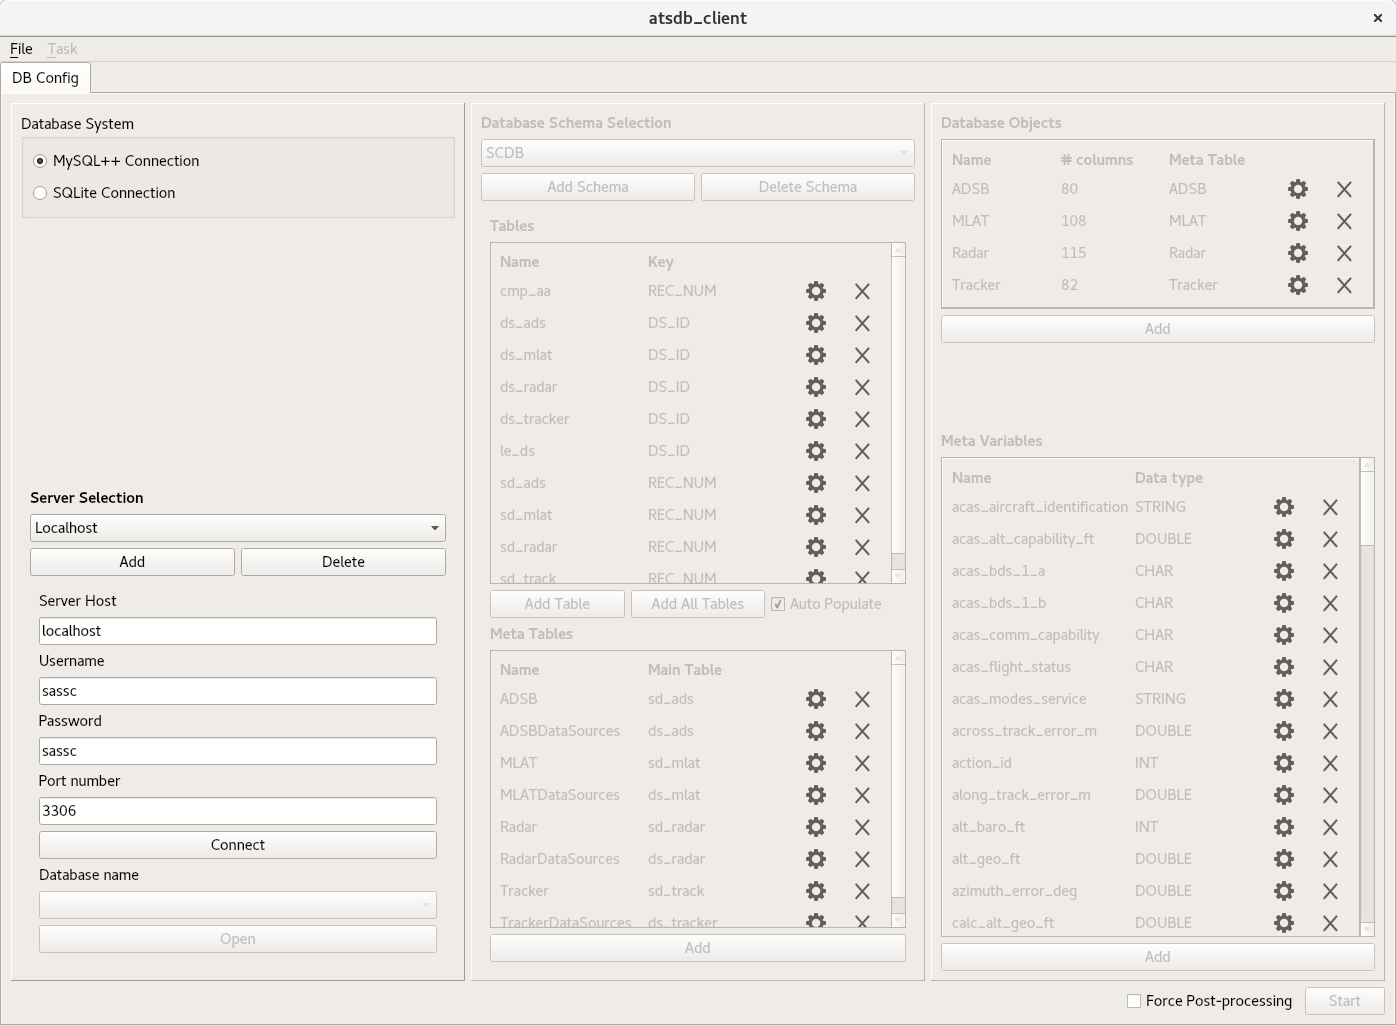
\includegraphics[width=18cm,frame]{../screenshots/db_config_connect.png}
  \caption{Connecting to a database}
  \label{fig:db_connect}
\end{figure}

On the left-hand side, a database system can be selected.  Choices are either MySQL database or a file container with a SQLite3 database. \\
On the lower left (depending on the database system) either a MySQL server connection can be configured or a list of SQLite3 files is shown.\\

On the right-hand side a database schema can be selected and edited (editing is only recommended for experienced users).

\subsection{Connecting to a MySQL Server}

\begin{figure}[H]
  \center
    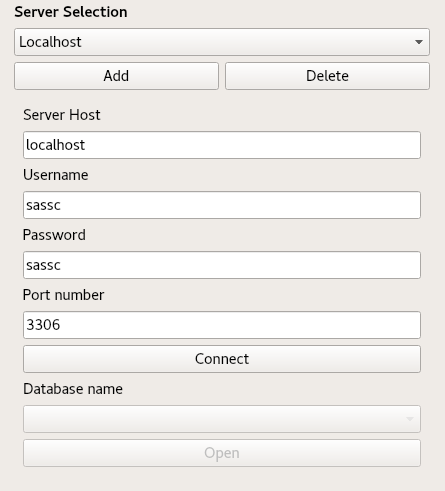
\includegraphics[width=7cm,frame]{../screenshots/mysql_server_selection.png}
  \caption{Connecting to a MySQL server}
  \label{fig:mysql_connect}
\end{figure}

Several MySQL servers can be defined, each one has a specific set of parameters. To add a new server, press the 'Add' button and enter a unique server name. To select the currently used server, use the dropdown menu. To delete the currently used server, press the 'Delete' button.

For connecting to a MySQL database, several parameters have to be entered:

\begin{table}[H]
  \center
  \begin{tabular}{ | l | l | l |}
    \hline
    \textbf{Parameter} & \textbf{Description} & \textbf{Example Values} \\ \hline
    Server Host & Network identifier of server & 'localhost', '10.0.0.123' \\ \hline
    Username & MySQL user name & 'sassc', 'root' \\ \hline
    Password & MySQL user password & 'sassc', '' \\ \hline
    Port Number & MySQL server port & '3306' \\
    \hline
  \end{tabular}
  \caption{MySQL server parameters}
\end{table}

To connect to a defined MySQL server, press the 'Connect' button.\\

\subsubsection{Access to SASS-C MySQL Servers}

Please note that it is not recommended to use SASS-C databases on which actual performance evaluations are to be performed. Using ATSDB, database operations can be performed which might impede results later obtained by using SASS-C. For this reason, it is recommended to either clone an evaluation or use one on which no later SASS-C evaluations are performed.

If a remote server is used, e.g. a SASS-C workstation, remote access might be prohibited, which will result in an access permissions error during connecting. To resolve this, (generally) remote access can be enabled in the servers MySQL configuration. As a superuser, edit the file 'my.cnf', which is commonly found under '/etc/mysql/my.cnf'. 

Find the line that states:
\begin{verbatim}
bind-address = 127.0.0.1
\end{verbatim}

Change the line to:

\begin{verbatim}
#bind-address = 127.0.0.1
\end{verbatim}

Then, restart the MySQL server using one the following commands:

\begin{verbatim}
/etc/init.d/mysqld restart

#OR, depending on your distribution
service mysql restart
\end{verbatim}

Then, to allow access to the databases, log into a MySQL client on the server as root and execute the following commands:

\begin{verbatim}
# log in as root, must be done as superuser
mysql -u root

# grant access rights for your MySQL user, 
# e.g. 'sass', from the your local IP address, 
# e.g. '192.168.0.104', using your password, e.g. 'sassc'
GRANT ALL ON *.* to 'sassc'@'192.168.0.104' IDENTIFIED BY 'sassc';

# set access rights
FLUSH PRIVILEGES;

# exit the MySQL client
exit
\end{verbatim}

After executing these steps once, remote access to this MySQL server from the specified IP address is enabled.

\paragraph{Firewall}

It might also be the case that your installation of SASS-C has an enabled firewall. If that is the case, access to be MySQL ports must be enabled.

\begin{figure}[H]
  \center
    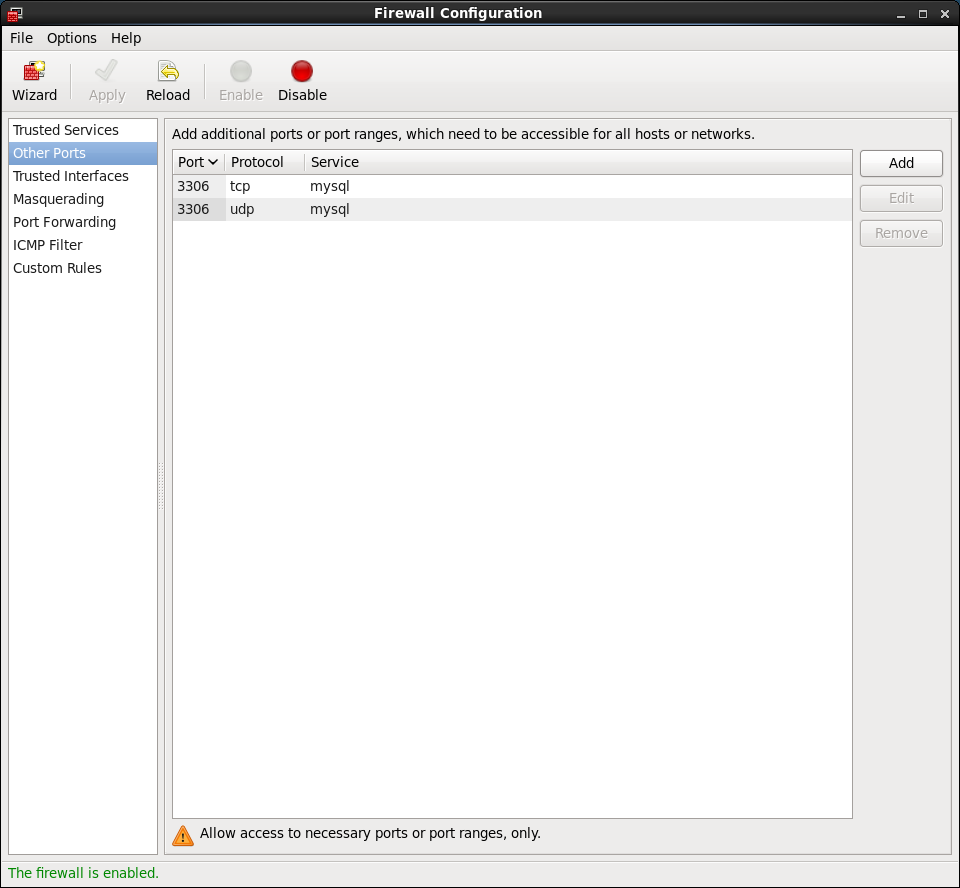
\includegraphics[width=15cm,frame]{../screenshots/centos_firewall.png}
  \caption{MySQL Server firewall example}
\end{figure}

\subsubsection{Error Messages}

If  a  wrong  database  name  or  IP  address  is  used,  error  messages  can  be  e.g.  \\

\begin{figure}[H]
  \center
    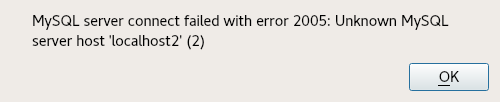
\includegraphics[width=9cm,frame]{../screenshots/mysql_connect_error.png}
  \caption{MySQL Server not found error.}
\end{figure}

 or 

\begin{figure}[H]
  \center
    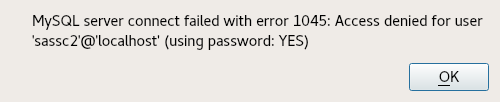
\includegraphics[width=9cm,frame]{../screenshots/mysql_user_error.png}
  \caption{MySQL user incorrect error.}
\end{figure}

If such an error occurs, correcting the server host name and or user/password should solve the problem.

\subsubsection{Opening a MySQL Database}

After successful connection, all existing databases in the server are shown in the 'Database name' drop-down menu. The last used one is selected automatically.

\begin{figure}[H]
  \center
    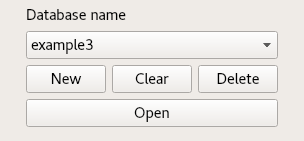
\includegraphics[width=5.5cm,frame]{../screenshots/mysql_database_selection.png}
  \caption{Selecting a MySQL database.}
  \label{fig:mysql_db_select}
\end{figure}

Several actions are available:

\begin{itemize}  
\item Drop-down selection: Selects the current database
\item New button: Allows creation of a new database
\item Clear button: Deletes all data with current database (after confirmation)
\item Delete button: Deletes current database (after confirmation)
\item Open button: Opens the current database
\end{itemize}

\subsubsection{Importing a MySQL Database}

After opening a database, import functions are available by clicking the 'Import' button:

\begin{figure}[H]
  \center
    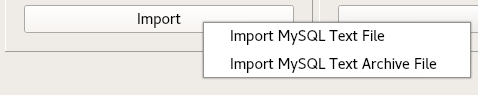
\includegraphics[width=9cm,frame]{../screenshots/database_import.png}
  \caption{Importing a MySQL database}
\end{figure}

\paragraph{Importing a MySQL Text File}

A previously exported MySQL database can be read from a text file and written into the current database. After selecting this option, a file open dialog is shown which allows selection of '*.sql' files. Please note the following points:

\begin{itemize}  
\item The text file must contain valid MySQL statements
\item MySQL functions/views are not imported, only data which can be inspected
\item If more than 3 errors occur during the import process, it is aborted
\item If the import process was aborted, the current database might contain already imported parts which are not deleted automatically
\end{itemize}

\paragraph{Importing a MySQL Text Archive File}

A previously exported MySQL database can be read from a text archive file and written into the current database. After selecting this option, a file open dialog is shown which allows selection of '*.tar.gz *.gz *.tar *.zip *.tgz *.rar' files. Please note the following points:

\begin{itemize}  
\item This function does \textbf{not} work to import an Verif-exported \textit{evaluation tgz}, but imports an \textit{SQL archive} from inside such an evaluation tgz
\item The text archive file must follow the same points as in the \textbf{Importing a MySQL Text File} section.
\item All files within the archive are read and imported into the database
\item If more than 3 errors occur during the import process, it is aborted
\item If the import process was aborted, the current database might contain already imported parts which are not deleted automatically
\end{itemize}

\paragraph{Importing a SASS-C Evaluation Export}

The following steps must be taken:

\begin{itemize}  
\item An export from a SASS-C evaluation must exist, e.g. 'example.tgz'
\item Using your favorite archive manager, extract the file 'tgz-tmp/<JOB\_NAME>/exported.sql.gz'
\item After successfully connecting to a server, create a new database, e.g. '<job\_name>', and open it
\item Click on the 'Import' button and select 'Import MySQL Text Archive File'
\item Select the previously extracted 'exported.sql.gz'
\end{itemize}

\subsubsection{SQlite3 File container}
\label{sec:sqlite_fc}
For opening a file container, clicking the 'Select' button opens a file selection dialog, in which any SQLite3 file can be selected as data source.

\begin{figure}[H]
  \center
    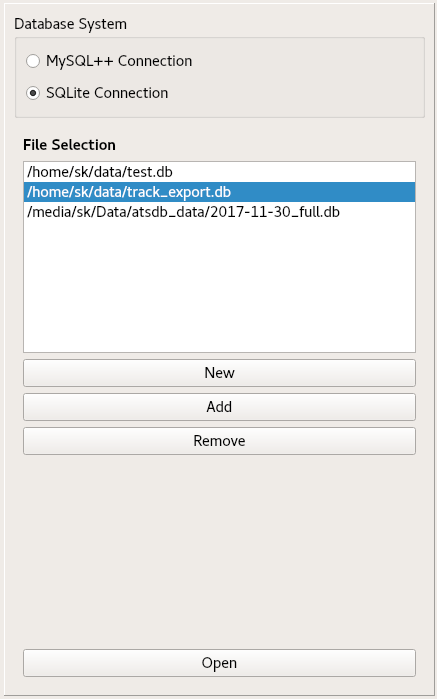
\includegraphics[width=8cm,frame]{../screenshots/sqlite3_open.png}
  \caption{Opening a SQLite3 file container}
  \label{fig:sqlite3_open}
\end{figure}

\subsection{Database Schema Selection}
For a common user, usage of the pre-configured database schema 'SCDB' is recommened. To select a different database schema, please use the 'Schema selection' drop-down menu.\\

\begin{figure}[H]
  \center
    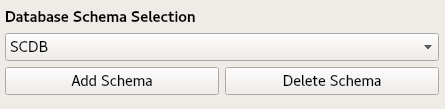
\includegraphics[width=8cm,frame]{../screenshots/database_schema_selection.png}
  \caption{Selecting a database schema}
  \label{fig:db_schema_select}
\end{figure}

For experienced users, a database schema can be created, edited and selected, which is currently not recommended (since it is not user friendly and might crash if used in the ``wrong'' manner).

Also, after locking the database schema, the existing Database Objects can be edited, which is currently also not recommended. There will be additional information about this subject in a later release, when the functionality has matured.

\begin{figure}[H]
  \hspace*{-1cm}
    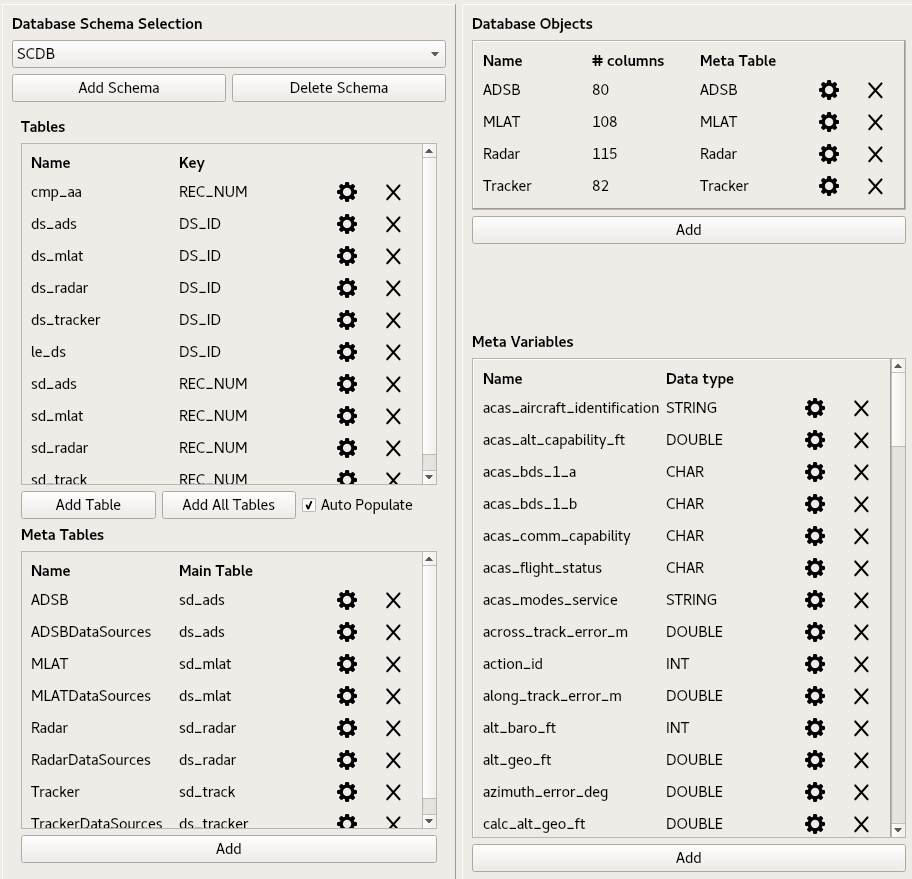
\includegraphics[width=16cm,frame]{../screenshots/database_schema_configuration.png}
  \caption{Configuring a database schema}
  \label{fig:db_schema_configuration}
\end{figure}

\subsection{Tasks}
\label{sec:tasks}

Since in SASS-C Verif radar plot coordinates are not given as latitude/longitude, which are the main coordinates for all processing in ATSDB, optionally these coordinates can be re-calculated and set in the database using the ''Calculate Radar Plot Position`` Task.

\subsubsection{Calculate Radar Plot Position}
To execute this task select ''Task``->  ''Calculate Radar Plot Position` in the top menu bar.

\begin{figure}[H]
  \center
    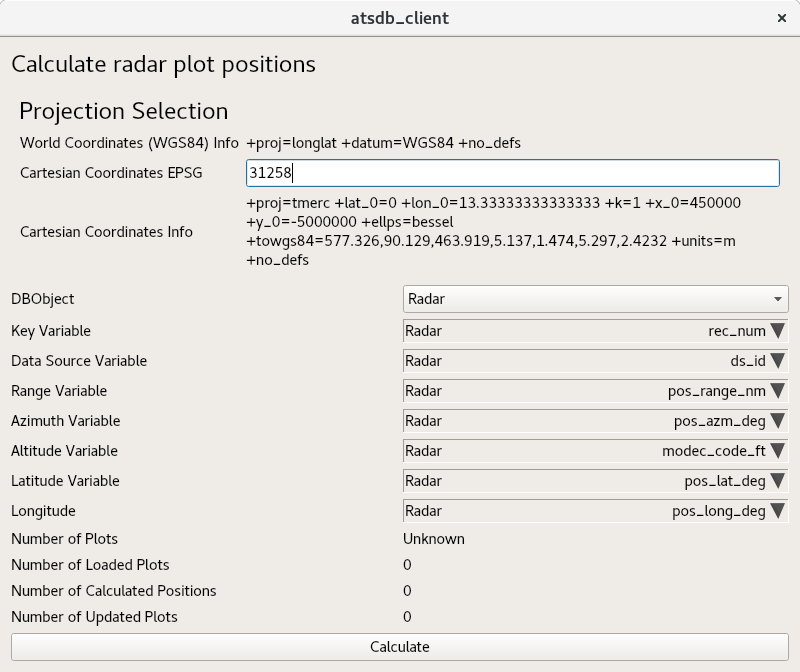
\includegraphics[width=14cm,frame]{../screenshots/task_calc_radar.png}
  \caption{Calculate radar plot position task}
  \label{fig:task_calc_radar}
\end{figure}

There are two projection methods (radar polar coordinates to WGS-84 coordinates) available. The \textit{RS2G} projection is the currently recommended option.

\paragraph{OGR Projection}

The EPSG code for the projection has to be chosen according to your needs, please refer to \url{http://spatialreference.org/ref/epsg/} for a list of possible codes.

The WGS84 latitude/longitude coordinates are then calculated using the radar positions in the database, the range and the azimuth. Please \textbf{note} that currently there will be offsets in the projected coordinates compared to the e.g. the ARTAS projection. The reason for this is under investigation.

\paragraph{RS2G Projection}

For this projection, no additional attributes must be given. Please \textbf{note} that while this projection is based on a common ``radar slant to geodesic transformation'', it is also not equivalent to e.g. the ARTAS projection. This will be improved in the near future, but validation was estimated to not to be taken lightly, and therefore the additional effort will be done before the next major release.

\paragraph{Calculation}

Press ``Calculate'' to start the calculation process, which will take a few minutes depending on the data size. \\

Messages like these will be printed in the text console, the last one indicates completion of the task:

The following windows will be shown, to give indication about the calculation progress:

\begin{figure}[H]
  \center
    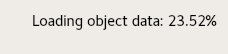
\includegraphics[width=4cm,frame]{../screenshots/task_calc_radar_load.png}
  \caption{Calculate radar plot position task: Loading}
\end{figure}

\begin{figure}[H]
  \center
    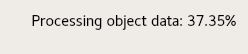
\includegraphics[width=4cm,frame]{../screenshots/task_calc_radar_process.png}
  \caption{Calculate radar plot position task: Processing}
\end{figure}

If there were projection errors in the calculation, the before insertion the user will be asked to confirm. The coordinates with projection errors will of course not be committed to the database, but will be skipped.

\begin{figure}[H]
  \center
    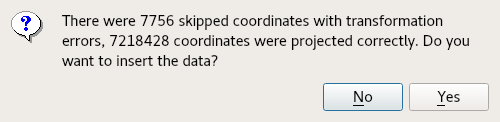
\includegraphics[width=9cm,frame]{../screenshots/task_calc_radar_insert.png}
  \caption{Calculate radar plot position task: Insertion question on errors}
\end{figure}


\begin{figure}[H]
  \center
    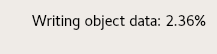
\includegraphics[width=4cm,frame]{../screenshots/task_calc_radar_write.png}
  \caption{Calculate radar plot position task: Writing}
\end{figure}

\begin{figure}[H]
  \center
    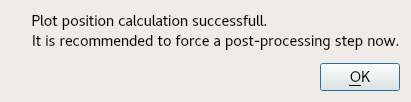
\includegraphics[width=8cm,frame]{../screenshots/task_calc_radar_done.png}
  \caption{Calculate radar plot position task: Done}
\end{figure}

After running this task once (per database), the radar plots also have a set latitude/longitude. As stated, a post-processing step is recommended after executing this task. \\

Please \textbf{note} that this task can be re-run with different projections if wanted.

Please \textbf{note} that no additional Radar plot information is changed, only the latitude/longitude variables are updated.
 

\subsection{Starting}

After the previous steps have been completed, the 'Start' button can be pressed to continue. \\

\begin{figure}[H]
  \center
    
\includegraphics[width=9cm,frame]{../screenshots/start.png}
  \caption{Starting}
\end{figure}

When a database is opened the first time, a post-processing will be performed automatically.

\subsubsection{Postprocessing}
When a database is imported, some information that eases usage of the software does not exist. This information is generated once during a post-processing step, which is automatically performed the first opening of a new database. If wanted, it can always performed using the 'Force post-processing' checkbox.

\begin{figure}[H]
  \hspace*{-2cm}
    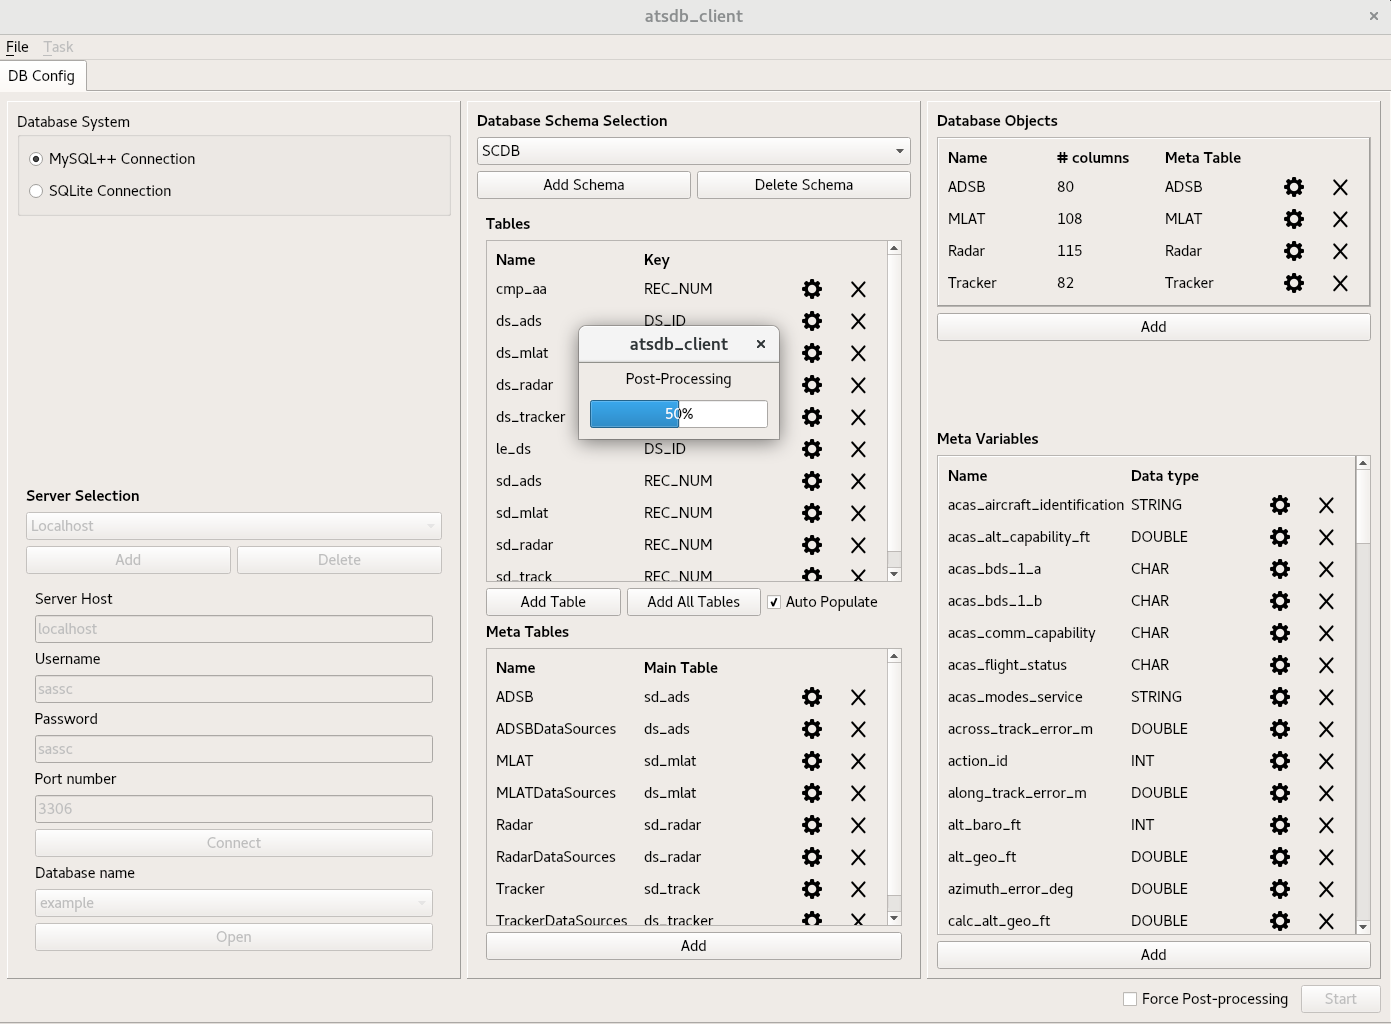
\includegraphics[width=18cm,frame]{../screenshots/db_postprocessing.png}
  \caption{Post-processing a database}
  \label{fig:db_postprocessing}
\end{figure}

The following information is generated and stored in the database:

\begin{itemize}  
\item List of all active data sources for all DBOs
\item List with all minima/maxima for all variables of all DBOs
\end{itemize}

Please \textbf{note} that this step has to be performed only once for each database, and may take up to a few minutes for large datasets. \\

Please also \textbf{note} that during this step, no DBO data itself is changed, but only additional information is generated and stored in separate database tables.
 
